\documentclass[runningheads]{llncs}

\usepackage{graphicx}
\usepackage{array}
\usepackage{booktabs}
\usepackage{float}
\usepackage{hyperref}
\usepackage{amsmath}
\usepackage{float}
\usepackage{subcaption}
\usepackage{color}

\renewcommand\UrlFont{\color{blue}\rmfamily}
% ---- Statistics ----- %
% abstract: 132
% Introduction: 554
% Related Work: 589

\begin{document}
    \title{Yet Another Problem of Automatic Evaluation of Generative Dialogue Systems}
    \titlerunning{Yet Another Problem}
    \author{Cong Feng\inst{1} \and Wenge Rong\inst{1}}
    \authorrunning{C. Feng et al.}
    \institute{
    School of Computer Science and Engineering, Beihang University, Beijing, China
    \email{cgsdfc@126.com} \\
    \email{w.rong@buaa.edu.cn}
    }

    \maketitle

    % --------------------------- %
    % --------- Abstract -------- %
    % --------------------------- %
    \begin{abstract}
        Evaluating generative dialogue systems with automatic metrics is a difficult problem. It has been shown that the word overlap metrics such as BLEU and the word embedding metrics correlate poorly with human judgments. In this paper, we highlight yet another problem of evaluation with metrics through an empirical study. We show that regardless of the correlation with human judgments, the scores of these metrics do not correlate well with one another, which means fine-tuning the system on one set of metrics may yield a gotcha when testing with another set of metrics. This infeasibility again adds to the ineffectiveness of evaluation done alone with metrics. To the end of utilizing metrics at its best, we offer several pragmatic suggestions on the use of automatic metrics to avoid the issue of metric inconsistency.
        \keywords{Automatic Metrics, Response Generation, Chatbot}
    \end{abstract}

    % ----------------------------------- %
    % ---------- Introduction ----------- %
    % ----------------------------------- %
    \section{Introduction}
    The chat-oriented dialogue systems have seen a boom in the recent literature of dialogue systems. These systems are trained to make an appropriate response given a conversational context and can be applied to various chatbot applications, language education tools, and intelligent personal assistants. This setting is different from that of the traditional task-oriented dialogue systems, which are programmed to assist their users on completion of a specific task, such as restaurant reservation and airline information acquisition. As a result, the chat-oriented dialogue systems cannot be evaluated in the same supervised setting as their task-oriented counterpart, which turns out to bring a new challenge.

    As an advanced approach to the chat-oriented system, the generative models based on neural networks feature end-to-end training with minimal hard-coded features and the ability to output fluent human-like sentences. Given a large corpus of context-response pairs, these neural models can learn language patterns and extract common-sense knowledge from the corpus in an unsupervised manner, making it a highly plausible solution to the response generation problem.

    The research community has made steady progress with the generative models. Vinyals et al. \cite{GoogleChatbot} applied the Seq2Seq model \cite{Seq2Seq} to generate responses to both technical queries in an IT helpdesk and open-ended questions such as \textit{what's the purpose of life?} Their model consistently outperformed a rule-based chatbot. However, generative models are not without problems. They incline to give meaningless responses to the questions they are incapable to handle, such as \textit{I don't know what you're talking about} and like any chat-oriented systems, their evaluation remains an open problem.

    Previous works of generative dialogue systems start by borrowing automatic metrics from the machine translation community, such as the popular BLEU \cite{BLEU} and METEOR \cite{METEOR}. However, the correlation between these borrowed metrics and human judgments remains unclear and researchers generally fall back to human evaluation for better accuracy and reliability \cite{Shang,DCGM,VHRED}. Liu et al. performed an empirical study on how well these automatic metrics correlate with human judgments \cite{HowNot}. They concluded that the metrics only correlated weakly with human judgments on the non-technical Twitter corpus and not at all on the technical Ubuntu Dialogue Corpus \cite{ubuntu_corpus}. They urged against the use of these metrics and called for the development of new automatic metrics that are more relevant to human judgments.

    In this paper, we extend the work of Liu et al.'s. and investigate the behaviors of automatic metrics when human judgments are not available. In particular, we highlight the drawbacks of existing metrics by trying to compare system performance purely based on them and show how inconsistent the results can be. Besides, we draw samples from the per-utterance scores of different metrics and analyze the pairwise correlation of these samples. We find that some pairs of samples have a high correlation, while other pairs show a much lower one.

    Following these observations, we cluster the metrics based on the pairwise correlations of their corresponding samples. The results show that metrics based on the same set of features tend to cluster together, indicating a high pairwise correlation within the same group. According to the experiment results, we argue that the scores from different metrics have the risk of high inconsistency, which is yet another pitfall of using automatic metrics. Therefore, it is strongly recommended to choose consistent metrics for the ease of comparison across different settings.

    % ----------------------------------- %
    % ----------- Related Work ---------- %
    % ----------------------------------- %
    \section{Related Work}
    Previous works on automatic metrics have mostly focused on the correlation between the metrics and human judgments. After all, the advantages of automatic metrics would be largely compromised if they cannot reflect human judgments. For example, in machine translation, where automatic metrics have been established to reduce human labor, almost every newly proposed metrics report an improved human correlation, as in \cite{NIST}, \cite{METEOR}, and \cite{chrf}.

    In dialogue response generation, to address the issue of low metric-human correlation, various semantic-based methods have been proposed. For example, the ADEM metric proposed by Lowe et al. models the human judgments with a feed-forward neural network \cite{ADEM}. Their concise architecture achieves a high correlation with human scores in various settings. The RUBER metric proposed by Tao et al. takes an asymmetric approach w.r.t the response-context pair and response-reference pair, where the former is modeled by a neural network and the latter is measured by an embedding-based metric. They combined two scores with various heuristics and achieved improvement on a Chinese corpus \cite{RUBER}. In brief, correlation with human judgments has always been the supervised signal guiding the evolution of automatic metrics.

    On the other hand, automatic metrics have been constantly doubted of their capability to reflect human judgments. In one of the earliest attempts to the response generation problem, Ritter et al. made an initial examination on the suitability of BLEU to this field leveraging the human data they collected \cite{Ritter11}. They found that the BLEU scores were very low even on the system level and the correlation was modest. Shang et al. argued that BLEU did not apply as the reasonable responses are too vast for the references to cover \cite{Shang}.

    Another popular metric is perplexity, which is generally used to evaluate statistical language models. Vinyals et al. showed that their Seq2Seq dialogue model achieved a much lower perplexity than the n-gram baseline, but they also admitted the drawbacks of using such a metric \cite{GoogleChatbot}. Serban et al. also used perplexity to evaluate their models in \cite{HRED}, along with other metrics. Like in \cite{GoogleChatbot}, they were not clear about how well these metrics accounted for the grammatical correctness and semantic coherence of the responses.

    An extensive study of metric-human correlation was conducted by Liu et al. \cite{HowNot}. Their study took into account of various settings, such as both retrieval and generative models and both technical and non-technical datasets. It revealed that although these metrics can distinguish state-of-art models from baseline models, none of them correlate highly with human scores. Their work has left us two questions towards better automatic metrics:
    \begin{enumerate}
        \item How can we improve the metric-human correlation?
        \item Why do the existing metrics correlate badly with human judgments?
    \end{enumerate}
    Previous works that proposed enhanced metrics endeavored to answer the first question, while we try to shed some light on the second one. In particular, we are curious about what can we learn when the scores from different metrics are put together and compared across various settings.

    To understand why some metrics correlate poorly with human judgments, we show that there are general inconsistencies among these metrics. Intuitively, if a set of metrics have low pairwise correlations, it is less likely that all of them would correlate highly with human judgments, which indicates that some of them must correlate poorly with human judgments. Along this line of thought, we arrive at an intermediate explanation to the poor performance of automatic metrics, backed by an empirical study. With this in mind, we can partially understand why these metrics fail and make improvements from the lesson we learned.

    % ----------------------------------- %
    % --------- Experiment Setup -------- %
    % ----------------------------------- %
    \section{Experiment Setup}
    Our experiment essentially involves training multiple generative models on multiple datasets, and then measure their performances with various automatic metrics. As stated, our study does not involve human evaluation. We also do not consider retrieval models as our interest falls on the more expressive generative models. Due to the constrains on time and resources, we limit our scope to three models and three datasets.

    To ease our demonstration, we define some symbols. A \emph{model} denoted as $m$ is an architecture of generative models, not an \emph{instance} of model trained on a specific dataset. A \emph{dataset} denoted as $d$ is a collection of context-response pairs from a specific domain, such as a social media or a technical support forum. A model predicts the response based on the context. A \emph{metric} denoted as $s$ is a function mapping a segment of words to a real value. The segment can be a sentence or a collection of sentences. The instance of model $m$ trained on dataset $d$ is denoted as $(m, d)$.

    % ------------------------- %
    % --------- Metrics ------- %
    % ------------------------- %
    \subsection{Metrics}
    We employ largely the same set of metrics studied by \cite{HowNot}, adding some novel ones from the recent literature. The word overlap and word embedding metrics, despite their issues with response generation, are studied again for more insights to their low performaces.

    \paragraph{BLEU.}
    BLEU \cite{BLEU} is a classical metric in the machine translation field that reports a high correlation with human scores on the system level. It owes the quality of a hypothesis to its similarity to a number of references and computes the similarity by accumulating n-gram precision of consecutive orders with the geometric mean, normalized by a brevity penalty.
    \begin{align}
        p_n &= \frac{ |C_n \cap R_n| }{ |R_n| } \\
        \textit{BP} &=
        \begin{cases}
            \ 1 \ & \text{if} \  c > r \\
            \ e^{1 - r/c} \ & \text{otherwise} \\
        \end{cases} \\
        \textit{BLEU} &=
        \textit{BP} \cdot \exp \left( \sum_{n=1}^N w_n \log p_n \right)
    \end{align}
    $p_n$ is the n-gram precision for order $n$. $C_n$ is a multiset of n-gram from a hypothesis while $R_n$ is the union of multisets of n-gram from each reference. $\textit{BP}$ is the brevity penalty. $c$ and $r$ are the length of the hypothesis and the effective length\footnote{The effective length of a collection of references is the length closest to that of the hypothesis.} of the references, respectively. $N$ is the total number of orders to compute n-gram precision for and a common choice is 4. $w_n$ is a weighting factor that usually takes the uniform weight $1 / N$.

    \paragraph{METEOR.}
    METEOR \cite{METEOR} is a metric proposed to address several issues with BLEU. It applies multiple stages of unigram matching to the hypothesis and reference, each using a different criterion, such as exact matching, WordNet synonyms, and paraphrases. An alignment is then created from these unigram matches. The score is based on the F1 score of the alignment and a penalty on shorter matches.

    \paragraph{ROUGE.}
    ROUGE \cite{ROUGE} is a family of metrics for automatic summarization. It defines a framework based on the F1 score and can integrate different matching units. For example, ROUGE-N uses n-gram as matching unit and ROUGE-L uses the longest common subsequence. The common form of ROUGE is:
    \begin{align}
        \textit{ROUGE} = \frac{
        R \cdot P
        }{(1 - \alpha) P + \alpha R}
    \end{align}
    with $R$ being the recall and $P$ being the precision. $\alpha$ controls the relative importance of $R$ and $P$, and it should be a large value if only recall is considered.

    \paragraph{Embedding Average.}
    Embedding Average is a metric based on word embedding, a distributed approach to the meaning of words \cite{word2vec}. The embedding of a sentence is defined as the average of the embeddings of its composing words. The similarity of two sentences is then simply defined as the cosine of the corresponding vectors:

    \paragraph{Vector Extrema.}
    Vector Extrema \cite{Vector_Extrema} composes the sentence embedding by taking the most extreme value (either maximum or minimum) along each dimension from its constituted words. The intuition is that in the embedding space, common words like function words are pulled towards the origin as they appear in the context of many different words, while informative words are pushed away from the origin in either positive or negative direction, since they tend to appear in more specific context. By taking the most extreme values from the embeddings of the constituted words, this method essentially captures the most informative words of a sentence and ignore common words.

    \paragraph{Greedy Matching.}
    Greedy Matching \cite{GreedyAndOptimal} is an embedding-based method without explicitly calculating a sentence vector. Instead, the two sentences under comparison are treated as a weighted bipartite graph, with their words as nodes and the embedding cosine of a pair of words $(w, w')$ as the weight of this edge. Greedy Matching is based on a greedy method to solve the optimal matching problem:
    \begin{align}
        G(r, \hat{r}) = \frac{
        \sum_{w \in r} \max_{\hat{w} \in \hat{r}} \cos(e_w, e_{\hat{w}})
        }{ |r| } \\
        \textit{Greedy-Matching} = \frac{
        G(r, \hat{r}) + G(\hat{r}, r)
        }{2}
    \end{align}
    where $r$ and $\hat{r}$ are the reference and response, respectively.

    \paragraph{ADEM}
    ADEM \cite{ADEM} is based on a nueral network, which is trained on a conversation corpus with human-annotated scores. The model first embeds the input into a low-rank vector space and then predicts a human score with a linear combination of the embeddings for a context $c$, response $\hat{r}$, and reference $r$.
    \begin{align}
        s(c, r, \hat{r}) = \frac{(c^T M \hat{r} + r^T N \hat{r} - \alpha)}{\beta}
    \end{align}
    $M, N$ are learnable parameters of the network and $\alpha, \beta$ are constants to normalize the output of the network to the five-point score. The model is trained end-to-end to minimize a squared error with a L2 regularization term:
    \begin{align}
        L = \sum_{i=1}^{K} (s_i - h_i)^2 + \gamma \left\| \theta \right\| _2
    \end{align}
    where $K$ is the number of samples in a batch. $s_i$ and $h_i$ are the score predicted by the model and the score labeled by human, respectively. $\theta$ is the parameters of the network and $\gamma$ is the regularization factor.

    \paragraph{Distinct-N.}
    Distinct-N \cite{MMI} measures the rate of unique n-grams of a sentence. For a sentence, it is the size of the set of the n-grams (each n-gram appears only once) divided by the total number of n-grams. It measures the diversity of a response at the token level.

    % ------------------------- %
    % --------- Models -------- %
    % ------------------------- %
    \subsection{Models}
    We choose the models used in \cite{VHRED}, namely LSTM, HRED, and VHRED. These models are either derived from the LSTM recurrent neural network \cite{LSTM} or extensions to the standard Seq2Seq framework. As such, they are ideal representatives of the generative models and have been widely used as baselines in various settings.

    \paragraph{LSTM.}
    The LSTM model is a simple generative model with a single RNN acting as both an encoder and a decoder. For an input sequence $X = x_1, x_2, \dots, x_n$ and an output sequence $Y = y_1, y_2, \dots y_m$, the model predicts $y_t$ conditioned on $x_t$ at time step $t$, as shown in figure \ref{fig:LSTM_as_generative}. Note that the generative LSTM is not an autoregressive model as the output of the previous time step does not become the input of the current time step.
    \begin{figure}
        \centering
        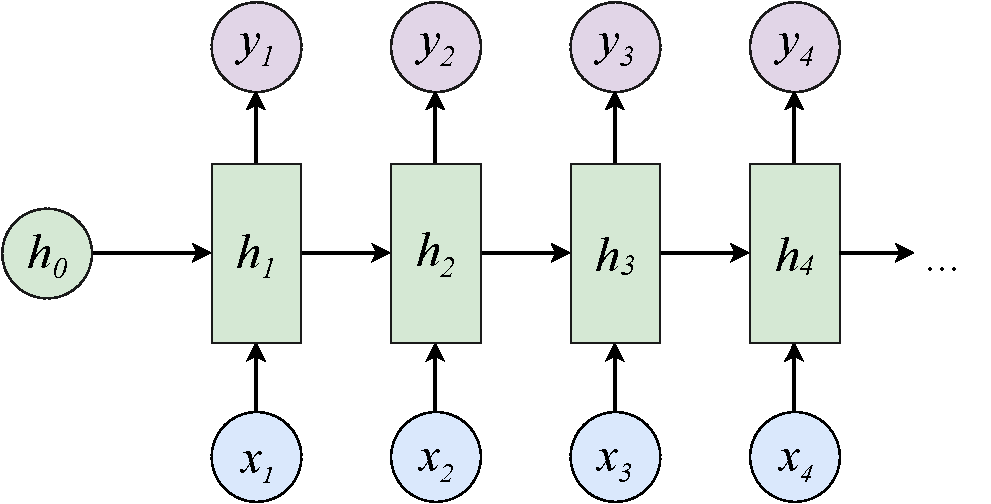
\includegraphics[width=0.5\textwidth]{figure/LSTM/generative.pdf}
        \caption{LSTM as a generative model}
        \label{fig:LSTM_as_generative}
    \end{figure}

    \paragraph{HRED.}
    The HRED model \cite{hred-qs,HRED} features a hierarchical encoding mechanism that takes into account the hierarchical structure of dialogues. For a dialogue $D$ with $M$ sentences: $D = U_1, U_2, \dots, U_M$, where each sentence $U_m$ consists of $N_m$ tokens: $U_m = w_{m, 1}, w_{m, 2}, \dots, w_{m, N_m}$, HRED first encodes each sentence with a \emph{utterance encoder} into a fixed-length utterance vector $e_u$. Then, these utterance vectors are processed iteratively by the \emph{context encoder} to produce a fixed-length context vector $e_d$. Finally, the \emph{utterance decoder} takes the context vector and generates the next utterance of the dialogue. With the hierarchical generation process, HRED can better incorporate long-term dialogue history and generate more topic-relevant resposnes \cite{A_Short_Review}.

    \paragraph{VHRED.}
    The VHRED model \cite{VHRED} extends the HRED model with a variational inference mechanism. Essentially, VHRED injects into the utterance decoder a random variable sampled from a high-dimension normal distribution, whose parameters are conditioned on the context vector $e_d$. With the randomness at the decoder, VHRED is able to model the uncertainty and ambiguity in the dialogues, generating more diverse responses.

    % --------------------------- %
    % --------- Datasets -------- %
    % --------------------------- %
    \subsection{Datasets}
    To observe a general phenomenon, we choose datasets from a variety of domains. Specifically, the technical domain is selected because it contains a lot of rare words and requires technical knowledge. The movie domain is selected for its fiction nature and dependencies on story backgrounds. The forum domain is selected since it reflects the disscusion around a specific topic with multiple participants.

    \paragraph{Ubuntu Dialogue Corpus}
    The Ubuntu Dialogue Corpus \cite{ubuntu_corpus} is a large-scale multi-turn dyadic technical corpus collected from the Ubuntu channel of an IRC network. It contains a lot of technical symbols, such as filesystem paths, commands, and URLs. Its technical nature with large number of examples helps construct data-driven applications for technical support.

    \paragraph{OpenSubtitles}
    The OpenSubtitles dataset \cite{opensub} is a large-scale monolingual corpus of movie subtitles. It is collected by the OPUS project \cite{OPUS} from the \emph{opensubtitles} website\footnote{\url{http://www.opensubtitles.org}}. It is noisy as its examples are inherently not of dialogue structure. In other words, there are no explicit turn-taking information or dialogue boundaries in it. Typically, the consecutive two utterances are treated as a context-response pair, as in \cite{GoogleChatbot}, \cite{MMI}, and \cite{persona}.

    \paragraph{LSDSCC}
    LSDSCC \cite{LSDSCC} is a \emph{Large Scale Domain-Specific Conversation Corpus} collected from the movie subreddit of the Reddit forum. It is believed that a more specific domain can help avoid generating universal responses \cite{LSDSCC}. The authors applied dedicated cleansing procedures to the raw data to retain as much information as possible. They also used human annotations to ensure the quality of the corpus.

    % ------------------------------------- %
    % --------- Experimental Study -------- %
    % ------------------------------------- %
    \section{Experimental Study}
    \subsection{System-Level Scores}
    We first measured system-level scores for all settings, shown in table \ref{tab:system_scores}. For the sake of space, each name in the table is abbreviated to its unique prefix, such as BLEU to BL, ROUGE to RO, and METEOR to MET, etc. A system-level score reflects the average performance of a model trained on a dataset. For inherently system-level metrics such BLEU, we directly compute them, while for other metrics, we compute the arithmetic average of their utterance-level scores.
    \begin{table}%
    \centering%
    \caption{System-Level Scores for All Settings}%
    \small
    \label{tab:system_scores}%
    \setlength{\tabcolsep}{0.11cm}%
    \begin{tabular}{|l|r|r|r|r|r|r|r|r|r|}%
        \hline
        & \multicolumn{3}{c|}{LSDSCC} & \multicolumn{3}{c|}{OpenSubtitles} & \multicolumn{3}{c|}{Ubuntu}\\%
        \hline
        & HRED & LSTM & VHRE & HRED & LSTM & VHRE & HRED & LSTM & VHRE\\%
        \hline%
        ADEM & \textbf{2.6178} & 2.6127 & 2.6163 & \textbf{2.6228} & 2.6224 & 2.6219 & 2.6353 & \textbf{2.6381} & 2.635\\\hline
        BL{-}1 & \textbf{0.08} & 0.0726 & 0.0722 & 0.0672 & 0.0638 & \textbf{0.0753} & 0.1314 & 0.1303 & \textbf{0.1365}\\\hline
        BL{-}2 & \textbf{0.0264} & 0.0181 & 0.0185 & 0.0171 & 0.0153 & \textbf{0.0264} & 0.0362 & 0.0345 & \textbf{0.0375}\\\hline
        BL{-}3 & \textbf{0.0105} & 0.0052 & 0.0066 & 0.0062 & 0.0055 & \textbf{0.0146} & \textbf{0.009} & 0.007 & 0.0089\\\hline
        BL{-}4 & \textbf{0.0053} & 0.0 & 0.0028 & 0.0024 & 0.0022 & \textbf{0.01} & \textbf{0.0029} & 0.0018 & 0.0025\\\hline
        Dist{-}1 & \textbf{0.9577} & 0.9441 & 0.9558 & \textbf{0.973} & 0.9714 & 0.9714 & 0.9074 & \textbf{0.9257} & 0.9113\\\hline
        Dist{-}2 & \textbf{0.8541} & 0.8511 & 0.8497 & \textbf{0.8669} & 0.8594 & 0.8665 & \textbf{0.9013} & 0.8603 & 0.8968\\\hline
        Greedy & \textbf{0.3303} & 0.3292 & 0.3267 & 0.3102 & 0.2998 & \textbf{0.3145} & \textbf{0.2775} & 0.2364 & 0.273\\\hline
        Average & \textbf{0.5532} & 0.5467 & 0.5483 & 0.5453 & 0.5295 & \textbf{0.5485} & \textbf{0.574} & 0.5205 & 0.5655\\\hline
        Extrem & \textbf{0.2841} & 0.2835 & 0.2814 & 0.3009 & 0.2929 & \textbf{0.3061} & \textbf{0.29} & 0.2663 & 0.2875\\\hline
        MET & \textbf{0.0296} & 0.0258 & 0.0281 & 0.0248 & 0.0233 & \textbf{0.0271} & 0.1657 & 0.1635 & \textbf{0.166}\\\hline
        RO{-}1 & \textbf{0.108} & 0.083 & 0.0978 & 0.0784 & 0.075 & \textbf{0.0872} & 0.1644 & \textbf{0.1836} & 0.1683\\\hline
        RO{-}2 & \textbf{0.0226} & 0.0049 & 0.0081 & 0.0053 & 0.0043 & \textbf{0.0107} & 0.0128 & \textbf{0.0143} & 0.0128\\\hline
        RO{-}3 & \textbf{0.0057} & 0.0002 & 0.0035 & 0.0011 & 0.0009 & \textbf{0.0053} & \textbf{0.0007} & 0.0003 & 0.0005\\\hline
        RO{-}4 & 0.0011 & 0.0 & \textbf{0.003} & 0.0002 & 0.0002 & \textbf{0.0038} & \textbf{0.0002} & 0.0 & 0.0001\\\hline
        RO{-}L & \textbf{0.0956} & 0.0681 & 0.0846 & 0.0742 & 0.0707 & \textbf{0.0826} & 0.1493 & \textbf{0.1722} & 0.1535\\\hline
        RO{-}W & \textbf{0.0792} & 0.0537 & 0.07 & 0.066 & 0.0629 & \textbf{0.0734} & 0.1205 & \textbf{0.1391} & 0.1236\\\hline
        PPL & \textbf{32.5599} & 32.9229 & 37.7149 & 41.6392 & 34.2724 & \textbf{33.6867} & \textbf{39.178} & 46.4061 & 40.2641\\\hline
        \#words & 13.1605 & 14.0067 & 12.3612 & 8.807 & 8.6394 & 8.7798 & 23.0646 & 16.4905 & 21.2449\\
        \hline
        %
        %
    \end{tabular}
    %
\end{table}

    \section{Discussion}
    Conclusions from the experiment.
    Advice on using metrics.

    \subsection*{Acknowledgements.}
    This work was done when the author has just graduated from Beihang University. The continuous support from the laboratory of Beihang University is the key to the completion of the work. The author also appreciates the encouragement and advice from his tutor Wenge Rong, an associate professor at Beihang University.

    \bibliographystyle{splncs04}
    \bibliography{data/all}
\end{document}
